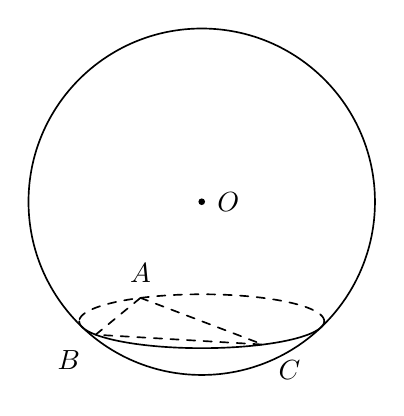
\begin{tikzpicture}[line width=.6pt, line join=round, line cap=round]

\coordinate (O) at (0,0);
\coordinate (A) at ({-2.2/sqrt(2)*cos(60)},{-2.2/sqrt(2)*sqrt(1-.22*.22)+.22*2.2/sqrt(2)*sin(60)});
\coordinate (B) at ({-2.2/sqrt(2)*cos(30)},{-2.2/sqrt(2)*sqrt(1-.22*.22)-.22*2.2/sqrt(2)*sin(30)});
\coordinate (C) at ({2.2/sqrt(2)*cos(60)},{-2.2/sqrt(2)*sqrt(1-.22*.22)-.22*2.2/sqrt(2)*sin(60)});
\draw (O) circle (2.2);
\draw[domain=180:360,samples=90,variable=\t] plot ({2.2/sqrt(2)*cos(\t)},{-2.2/sqrt(2)*sqrt(1-.22*.22)+.22*2.2/sqrt(2)*sin(\t)});
\draw[dashed,domain=0:180,samples=90,variable=\t] plot ({2.2/sqrt(2)*cos(\t)},{-2.2/sqrt(2)*sqrt(1-.22*.22)+.22*2.2/sqrt(2)*sin(\t)});
\draw[dashed] (A)--(B)--(C)--cycle;
\fill (O) circle (1.2pt);
\node[right=2pt] at (O) {$O$};
\node[above=2pt] at (A) {$A$};
\node[below left=2pt] at (B) {$B$};
\node[below right=2pt] at (C) {$C$};
\end{tikzpicture}
